\documentclass [11 pt, twoside] {article}


\def \jtitle {Lie groups}
\def \jlecturer {Richard Borcherds}
\def \jterm {}
\def \jauthor {Jack DeSerrano}


\usepackage [course] {jack}

\title {Lie groups}
\author {Jack DeSerrano}

\begin {document}

\maketitle

These notes are based on Richard Borcherds's YouTube series on Lie groups.\footnote{See \url{https://www.youtube.com/playlist?list=PL8yHsr3EFj53RWBkiHKoOsTw-dGHAoJ-h}.}

\begin {figure}
	\begin {center}
		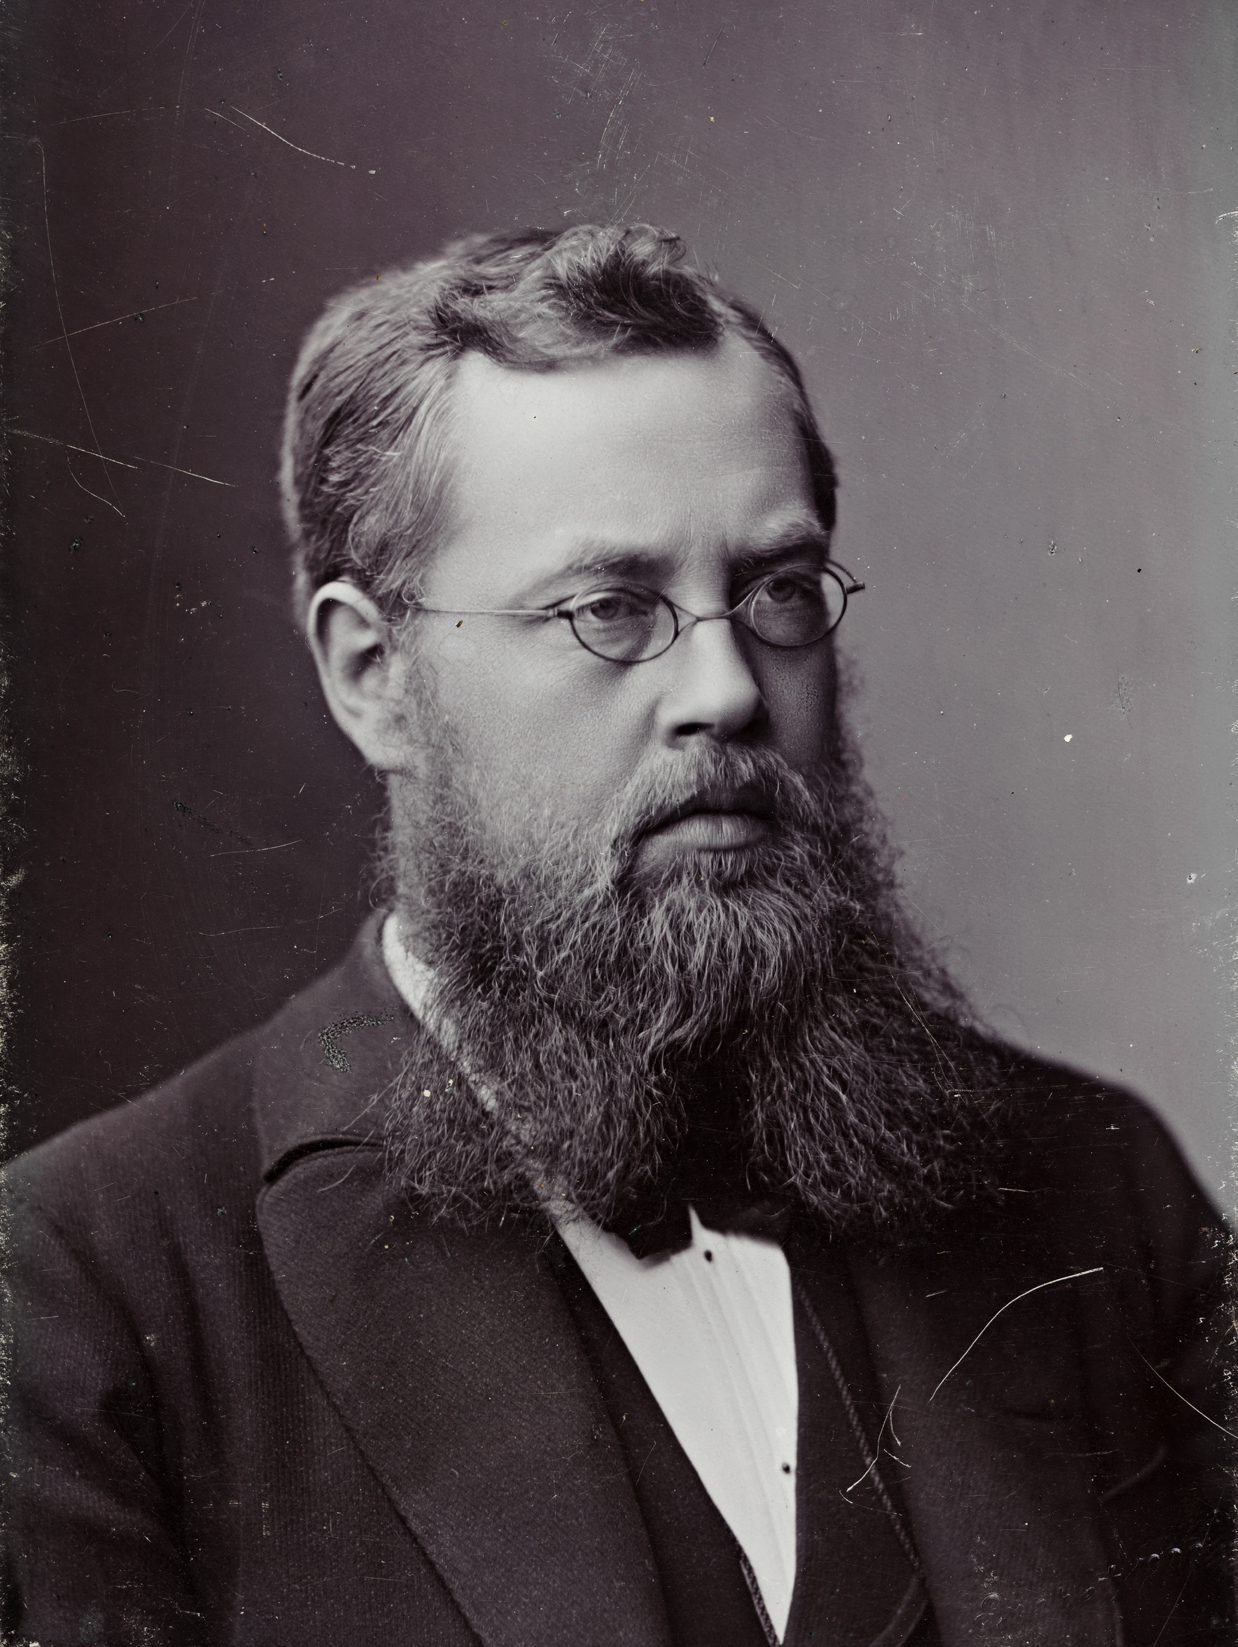
\includegraphics [scale = 0.33] {images/lie}
		\caption {Sophus Lie.}
	\end {center}
\end {figure}
% https://upload.wikimedia.org/wikipedia/commons/a/a3/Portrett_av_Sophus_Lie.jpg
% https://www.flickr.com/photos/48220291@N04/8447487830

\newpage

\iffalse
	\hypersetup {linkcolor = black}
	\tableofcontents
	\hypersetup {linkcolor = Red}
\fi

\section {Introduction}
First thing's first:
\begin{align*}
	\textrm{Lie} = \textrm{li\textlengthmark}
\end{align*}

A \defn{Lie group}\index{Lie group} is a group and a manifold, so, locally, it looks like $\mathbf{R}^{n}$. The number $n$ is the \defn{dimension}\index{dimension of a Lie group} of the Lie group.

The group $\GL_{n}(\mathbf{R})$ is a Lie group of dimension $n^{2}$: It is an open subset of the space of $n\times n$ matrices. 

Lie groups of dimension $0$ are, essentially, the same as discrete groups.
The classification of discrete groups is completely hopeless.
However, any Lie group $G$ has a connected component $G\sub{con}$ that is a normal subgroup of $G$.\footnote{This group is also a Lie group.}
The quotient $G\sub{disc} = G/G\sub{con}$ is $0$-dimensional.
Thus, one can split a Lie group into a discrete part and a connected part. One can, more or less, classify the connected Lie groups.

\begin{example}[ ]\label{}\text{}
Take $G:= \mathbf{R}^{*}$. 
Then, $G\sub{con} = \mathbf{R}_{>0}$ is the connected part and $G\sub{disc} = \{+,-\}$ is the discrete part.
\end{example}

The groups $\mathbf{R}$ under addition, $\mathbf{R}^{*}$ under multiplication, and $S^{1}\subset \mathbf{C}^{*}$ are $1$-dimensional Lie groups.
There are group homomorphisms
\[
\begin{tikzcd}
	\exp:\mathbf{R}\ar[r] & \mathbf{R}^{*}
\end{tikzcd}
\]
and
\[
\begin{tikzcd}
	\mathbf{R}^{*}\ar[r] & S^{1} : z\ar[r,mapsto] & e^{2\pi i z}.
\end{tikzcd}
\]
The second homomorphism is a \defn{local isomorphism}\index{local isomorphism}.
Any connected $1$-dimensional Lie group is isomorphic to $\mathbf{R}$ under addition or $S^{1}$ under multiplication.

Clearly, $\mathbf{R}^{1}\times \mathbf{R}^{1} = \mathbf{R}^{2}$, $\mathbf{R}^{1}\times S^{1}$, and $S^{1}\times S^{1}$ are $2$-dimensional Lie groups. 
Each of these Lie groups is of the form $\mathbf{R}^{2}/G\sub{disc}$ where $G\sub{disc}$ is a discrete group.\footnote{This group is $0$, $\mathbf{Z}$, or $\mathbf{Z}^{2}$.}
Any abelian connected Lie group is isomorphic to
\begin{align*}
	\mathbf{R}^{m} \times (S^{1}) ^{n} \isomto \mathbf{R}^{m+n}/G\sub{disc}
\end{align*}
where $G\sub{disc}$ is a discrete group.

There are no nonabelian connected Lie groups of dimension $1$. 
However, the $az+b$ group is a connected Lie group of dimension $2$, and one can see that it is nonabelian. Nevertheless, it is a \defn{solvable Lie group}\index{solvable Lie group}: That is, there is a chain of Lie groups
\begin{align*}
	1 = G_0 \subset \cdots \subset G_{n} = G
\end{align*}
where $G_{i}/G_{i-1}$ is abelian.

The group $\SL_{2}(\mathbf{R})$ is a dimension-$3$ Lie group. From this, one gets the $3$-dimensional Lie group
\begin{align*}
	\PSL_{2}(\mathbf{R}) = \SL_{2}(\mathbf{R}) / \left\{ \pm 1 \right\}.
\end{align*}
This is the group $\Aut(\mathfrak{H})$ via the action
\begin{align*}
	\mat{a&b\\c&d}(\tau) =  \frac{a\tau+b}{c\tau+d}.
\end{align*}
The group $S^{3}$, which one can think of as the unit quaternions, is a $3$-dimensional Lie group.\footnote{The sphere $S^{n}$ is a Lie group for $n=0,1,3$.}

The \defn{Heisenberg group}\index{Heisenberg group} 
\begin{align*}
	\underbrace{\mat{1&a&b\\&1&c\\&&1} }_{\mathbf{R}^{3}} / \underbrace{\mat{1&0&n\\&1&0\\&&1}}_{\mathbf{Z}} 
\end{align*}
is a Lie group of dimension $3$.\footnote{This is an example of taking a Lie group and modding out by a discrete subgroup of its centre.}
One can transform a function via
\[
\begin{tikzcd}[row sep = 0 em]
	f(z) \ar[r,mapsto] & f(z+a);\\
	f (z) \ar[r,mapsto] & e ^{icz}f(z);\\
	f (z)\ar[r,mapsto] & \alpha f (z);
\end{tikzcd}
\]
where $\left\lvert \alpha \right\rvert =1$.
These transformations correspond to elements of the Heisenberg group.
While $\mathbf{R}^{3}$ is simply connected, the Heisenberg group isn't. Nevertheless, its fundamental group is $\mathbf{Z}$.

One can reduce the classification of Lie groups to the classification of simply connected Lie groups: Any Lie group is a simply connected Lie group modulo a discrete subgroup of its centre. 

The Heisenberg group is \defn{nilpotent}\index{nilpotent group}. More generally, any group
\begin{align*} % https://tex.stackexchange.com/questions/17416/create-a-new-integral-symbol/17419#17419
	\mat{1&*&&*&*\\
		      &1&*& \hbox to .2em{\hss\scalebox{1}[1] {\rotatebox[origin=c]{90}{$\ddots$}}\hss} &*\\
		      &&\ddots&\ddots\\
		      &&&1&*\\
		      &&&&1} 
\end{align*}
is nilpotent.

The \defn{Lorentz group}\index{Lorentz group} $\O_{1,3}(\mathbf{R})$ is the group of rotations of spacetime: The group of linear operators on $\mathbf{R}^{4}$ that preserve the quadratic form
\[
\begin{tikzcd}
	(z_1,z_2,z_3,z_4)\ar[r,mapsto]& z_1^{2} - z_2^{2}-z_3^{2}-z_4^{2}.
\end{tikzcd}
\]
The Lorentz group is a $6$-dimensional Lie group that has a nontrivial fundamental group.
It has $4$ components: One can reverse time and reverse space.
Physicists believed that all physical theories were invariant under time reversal and space reversal. However, the weak interaction is not invariant under space inversion. Things do not need to be invariant under time inversion, either. 

The connected component of $\O_{1,3}(\mathbf{R})$ has a double cover $\Sp_{1,3}(\mathbf{R})$ called a \defn{spin group}\index{spin group}.
The group $\Sp_{1,3}(\mathbf{R})$ is locally isomorphic to $\SL_{2}(\mathbf{C})$, which has $2$-dimensional representations that $\O_{1,3}(\mathbf{R})$ does not have. This causes the existence of fermions and electrons.
This local isomorphism is an example of an ``accidental isomorphism.'' There are many ``accidental isomorphisms'' between Lie groups of small dimensions.

The group $\SU_3$ is an $8$-dimensional Lie group. This group is the gauge group of quantum chromodynamics and is involved in the flavour symmetries of old theories of the strong interaction.\footnote{Murray Gell-Mann called it the ``eightfold way.''}
This is a \defn{simple Lie group}\index{simple Lie group}: That is, it has no nontrivial connected normal subgroups.

The \defn{Poincar\'e group}\index{Poincar\'e group} $\mathbf{R}^{1,3} \rtimes \O_{1,3}(\mathbf{R})$ is a $10$-dimensional Lie group.
The Lie group $\mathbf{R}^{1,3}$ is solvable and the Lie group $\O_{1,3}(\mathbf{R})$ is a product of simple Lie groups.

Complex simple Lie groups are complex manifolds, not real manifolds. Examples of these include $\SL_{n}(\mathbf{C})$ for $n\ge 1$, $\O_{n}(\mathbf{C})$ for $n\ge 3$, and $\Sp_{2n}(\mathbf{C})$ for $n\ge 1$. These are the \defn{classical groups}\index{classical group} over $\mathbf{C}$.
Wilhelm Killing added $5$ more to this list:
\begin{center}
\begin{tabular}{ll}
    Group & Dimension\\
    \midrule
    $G_2$ & $14$\\
    $F_4$ & $52$\\
    $E_6$ & $78$\\
    $E_7$ & $133$\\
    $E_8$ & $248$
\end{tabular}
\end{center}
Dr. Borcherds remarks:
\begin{quote}
	\small Killing really ought to be a lot better known. He was a kind of really modest, shy guy and invented a lot of things that were later named after other people. Later on in this course, we will be talking about the Weyl group, the Coxeter number, the Cartan form, and things like that, and these were all actually first invented by Killing and people kind of forgot he invented them.
\end{quote}

\section {Lie algebras}
Lie groups---for example, $\GL_{n}(\mathbf{R})$---can be complicated.
One can replace the Lie group with the corresponding Lie algebra, which is much less complicated (it is a vector space).
One wants to put more structure on the Lie algebra so that it says something about the Lie group.

\begin{figure}
	\begin{center}
		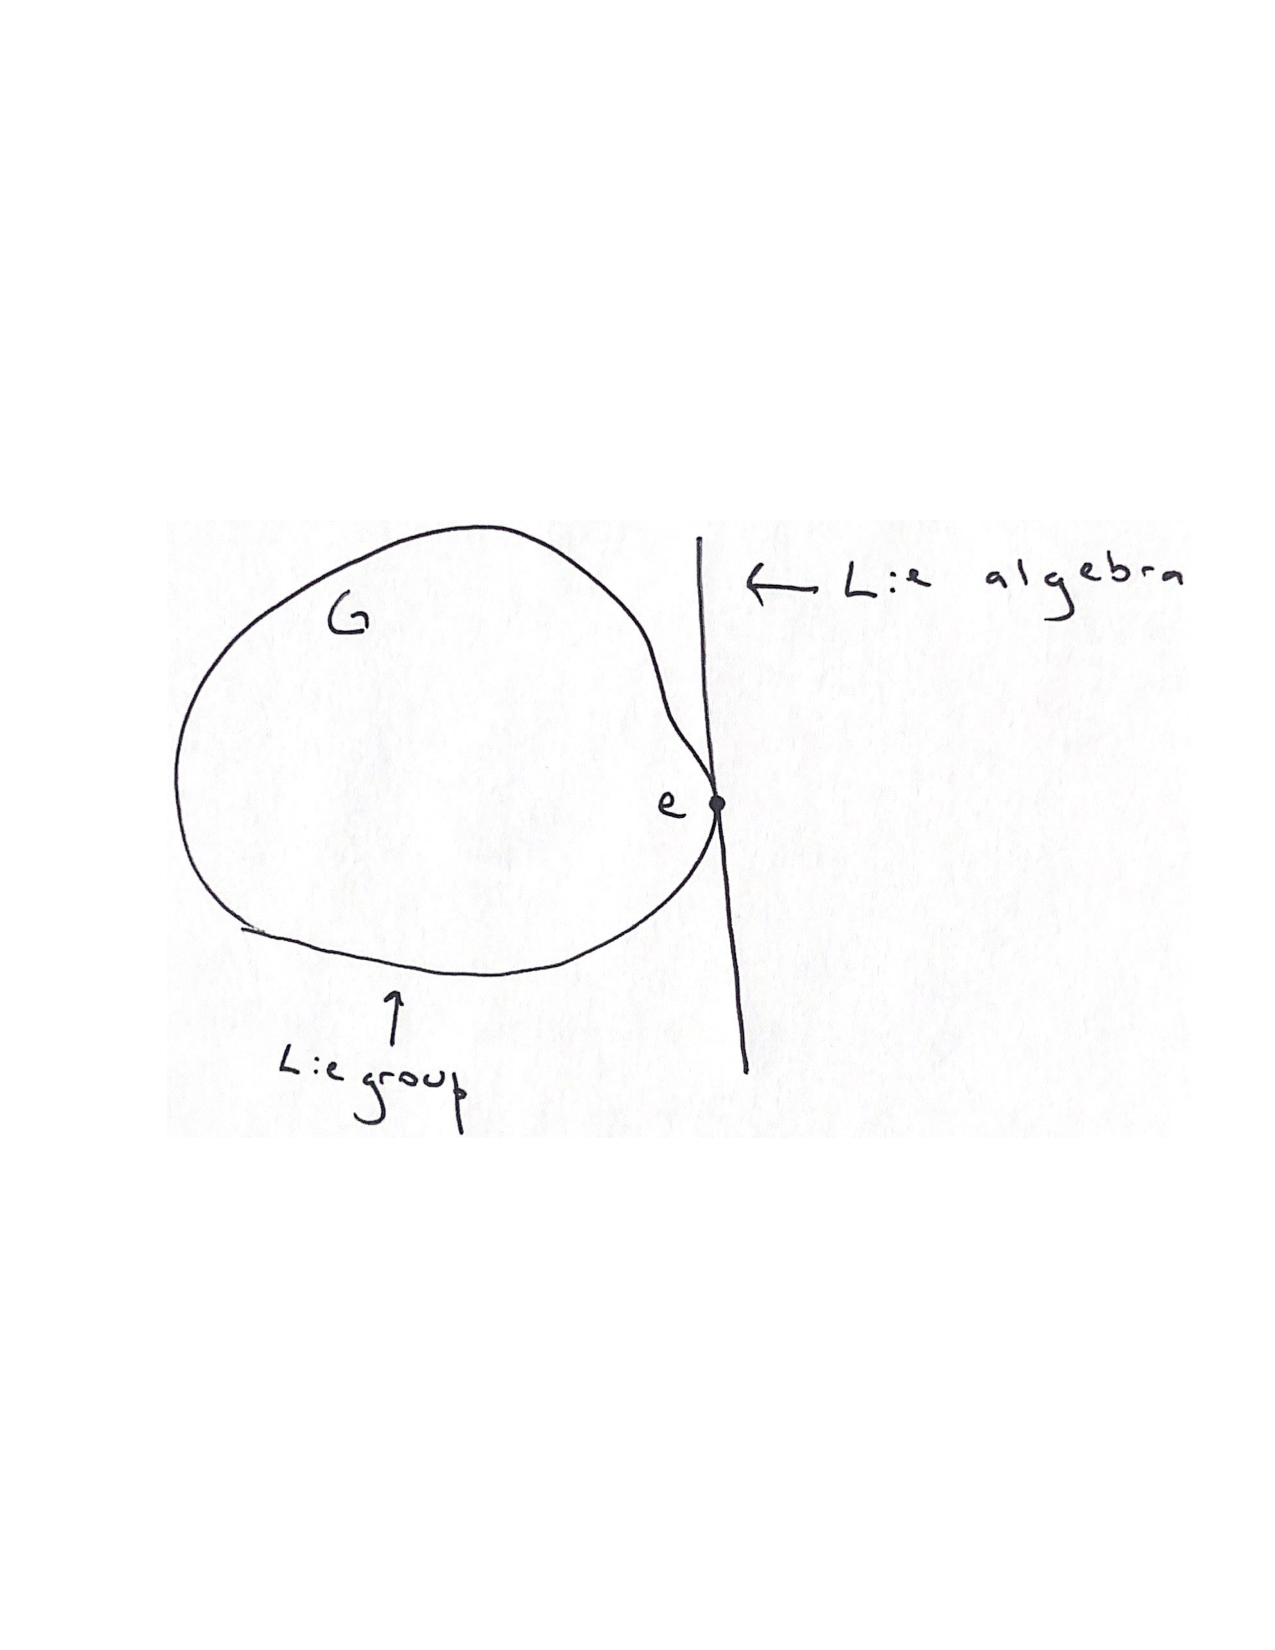
\includegraphics[scale=0.5]{images/tangentspace}
		\caption{The Lie algebra corresponding to a Lie group $G$ is the tangent space at the identity.}
	\end{center}
\end{figure}

A  \defn{first-order differential operator}\index{first-order differential operator} is a sum
\begin{align*}
	\sum_{i=1}^{d} f_{i}(X_1,\hdots,X_{d}) \frac{\partial}{\partial X_{i}}.
\end{align*}
First-order differential operators are, more or less, the same as vector fields on a manifold.
One can think of a vector field on a manifold as an infinitesimal automorphism that pushes each point an ``infinitesimal'' distance along the vector at that point.

Let $D = \sum_{i=1}^{d} f_{i}(X_1,\hdots,X_{d})\partial/\partial X_{i}$ and $E = \sum_{i=1}^{d} g_{i}(X_1,\hdots,X_{d})\partial/\partial X_{i}$ be first-order differential operators.
One can write
\begin{align*}
	D E &= \sum_{1\le i,j\le d}^{} f_{i} \frac{\partial}{\partial X_{i}} g_{j}\frac{\partial}{\partial X_{j}}\\
		 &= \sum_{1\le i,j\le d}^{} f_{i}g_{j}\frac{\partial}{\partial X_{i}}\frac{\partial}{\partial X_{j}} + f_{i}\frac{\partial g_{j}}{\partial X_{i}}\frac{\partial}{\partial X_{j}}.
\end{align*}
Similarly,
\begin{align*}
	ED &= \sum_{1\le i,j\le d}^{} f_{i}g_{j}\frac{\partial}{\partial X_{i}}\frac{\partial}{\partial X_{j}} + g_{j}\frac{\partial f_{i}}{\partial X_{j}} \frac{\partial}{\partial X_{i}}.
\end{align*}
Though $DE$ and $ED$ are not first-order, $DE-ED$ is first-order.
One can defines the \defn{Lie bracket}\index{Lie bracket} to be
\begin{align*}
	[D,E] := DE - ED.
\end{align*}

\begin{exercise}\label{}\text{}
Suppose that $D$ and $E$ are differential operators of orders $m$ and $n$ respectively.
Show that $[D,E]$ has order $m+n-1$.
\end{exercise}

One can see that 
\begin{align*}
	[D,E] = -[E,D].
\end{align*}
There is also the \defn{Jacobi identity}\index{Jacobi identity}:
\begin{align*}
	[[A,B],C] + [[B,C],A] + [[C,A],B] = 0.
\end{align*}
This is true for any (associative) ring.

\begin{definition}[ ]\label{}\text{}
A \defn{Lie algebra}\index{Lie algebra} $\mathfrak{g}$ is a vector space over $\mathbf{R}$ or $\mathbf{C}$ that has a bilinear map 
\begin{tikzcd}[cramped]
	{[}\ ,\ {]} : \mathfrak{g}\times \mathfrak{g}\ar[r]& \mathfrak{g}
\end{tikzcd}
that satisfies 
\begin{align*}
	[x,y] =- [y,x]
\end{align*}
and
\begin{align*}
	[[x,y],z] + [[y,z],x] + [[z,x],y] =0
\end{align*}
for all $x,y,z\in \mathfrak{g}$.
\end{definition}

\begin{remark}
	One can take $\mathfrak{g}$ to be a module over a commutative ring.
\end{remark}

Let $G$ be a Lie group with identity $e$. Let $T_{e}G$ be the tangent space to $G$ at $e$.
Notice that $G$ acts on itself by left translation. A left-invariant vector field on $G$ is uniquely determined by its value at $e$. That is, left-invariant vector fields on $G$correspond to tangent vectors to $G$ at $e$.
Vector fields correspond to first-order differential operators, so the left-invariant vector fields on $G$ are closed under the Lie bracket. Left-invariant vector fields correspond to tangent vectors to $G$ at $e$, so $T_{e}G$ has a Lie bracket. Thus, we define the Lie algebra of a Lie group $G$ to be 
\begin{align*}
	\mathfrak{g} := T_{e}G.
\end{align*}

\begin{example}[ ]\label{}\text{}
Consider $G =\mathbf{R}^{n}$ with addition.
The left-invariant vector fields on $G$ are of the form
\begin{align*}
	\sum_{i=1}^{n} a_{i} \frac{\partial}{\partial X_{i}}
\end{align*}
where $a_{i}$ is constant.
The Lie bracket of any two such operators is $0$, so the Lie algebra of $G$ is commutative. 
\end{example}

\iffalse
\begin{example}[ ]\label{}\text{}
Let $\mathfrak{g}$ be the Lie algebra of $G = \GL_{n}(\mathbf{R})$. The identity of $G$ is the identity matrix $e$, and the tangent space to $G$ at $e$ can be identified with $M_{n}(\mathbf{R})$.
Let $x\in M_{n}(\mathbf{R})$. What does the vector field $D$ corresponding to $x$ look like?
For a function $f$ on $\GL_{n}(\mathbf{R})$, this vector field is given by
\begin{align*}
	Df = \frac{f(a(1+\eps x)) - f(a)}{\eps}
\end{align*}
for $a\in G$.
This is the lowest order term of $f(a (1+\eps x)) - f(a)$, which is $\eps$ times something, which we want, plus higher order terms.

Let $x$ and $y$ be vector fields corresponding to differential operators $D$ and $E$ respectively.
Then, at $a\in G$, $(ED)f$ is the lowest order term of
\begin{align*}
	f(a(1+\delta y) (1+\eps x)) - f(a(1+\delta y)) - f(a(1+\eps x)) + f(a),
\end{align*}
which is $\eps\delta$ times something, which we want, plus higher order terms.
One sees that $(DE)f$ is similar and $(DE-ED)f$ is the lowest order term of 
\begin{align*}
	f(a(1+\eps x) (1+\delta y)) - f(a(1+\delta y) (1+\eps x)).
\end{align*}
Taking $a$ to $(1+\eps x-\delta y + \delta \eps yx)a$, this is the lowest order term of
\begin{align*}
	f(a(1-\delta\eps yx + \eps\delta xy)) - f(a),
\end{align*}
which is the differential operator corresponding to $xy-yx$. Thus, the Lie bracket of differentiable operators corresponding to matrices $x$ and $y$ is $xy-yx$, so we get the same bracket whether we consider $x$ and $y$ as matrices or left-invariant vector fields.  

It follows that the Lie algebra of $G$ is $\mathfrak{g} = M_{n}(\mathbf{R})$ with Lie bracket $[x,y] = xy-yx$.
For a closed subgroup of $\GL_{n}(\mathbf{R})$, the tangent space at $e$ is a subspace of $M_{n}(\mathbf{R})$ and the Lie bracket one gets is the restriction of the one above.
\end{example}

\begin{example}[ ]\label{}\text{}
Consider $G=\SL_{n}(\mathbf{R})$. Then, the tangent space $T_{e}G$ consists of matrices $x$ such that $\det(1+\eps x) = 1 + O (\eps^{2}) = 1 + \eps \tr(x) + \eps ^{2}\cdots$, so $\tr(x)=0$.
Thus, the Lie algebra of $\SL_{n}(\mathbf{R})$ is $n\times n$ matrices with trace $0$.
\end{example}

\begin{example}[ ]\label{}\text{}
Consider $G = O_{n}(\mathbf{R}) = \{x\in M_{n}(\mathbf{R}) : xx^{*}=e\}$. 
The tangent space $T_{e}G$ consists of matrices $x$ such that $(e+\eps x)(e+\eps x) ^{*}=  e + O(\eps^{2})$.
Since $(e+\eps x) (e+\eps x) ^{*} = e + \eps x + \eps x ^{*} + \eps ^{2}xx^{*}$, $T_{e}G$ (that is, the Lie algebra) consists of matrices with $x+x^{*}=0$.
\end{example}

One can compute the Lie algebra differently.
For example, let $G=\GL_{n}(\mathbf{R})$.
One defines $[x,y]$ to be the lowest-order term of the commutator $a^{-1}b^{-1}ab$ where $a\approx 1+\eps x$ and $b\approx 1+\delta y$ are elements of $G$ and $x$ and $y$ are tangent vectors. 
One sees that
\begin{align*}
	a^{-1}b^{-1}ab &= (1-\eps x) (1-\delta y)  (1+\eps x) (1+\delta y)\\
		       &= \eps\delta (xy-yx) + \textrm{higher order terms.}
\end{align*}
One gets the Jacobi identity here from the \defn{Hall--Witt identity}\index{Hall--Witt identity}:
\begin{align*}
	[[x,y^{-1}],z]^{y}[[y,z^{-1}],x]^{z}[[z,x^{-1}],y]^{x} = 1
\end{align*}
where $[x,y] = x^{-1}y^{-1}xy$ and $x^{y}=y^{-1}xy$.
\fi


\section {Lie groups and Lie algebras}
Note: we are working in the finite-dimensional case.

If two groups have the same Lie algebras, are they isomorphic?
A homomorphism of (Lie) groups \begin{tikzcd}[cramped]
	G\ar[r]& H
\end{tikzcd}
induces a homomorphism of the corresponding Lie algebras \begin{tikzcd}[cramped]
	\mathfrak{g}\ar[r]&\mathfrak{h}
\end{tikzcd}
that preserves the Lie bracket, but does a homomorphism of Lie algebras give a homomorphism of the corresponding Lie groups?
If $G$ is a closed subgroup of $H$, then $\mathfrak{g}$ is a subalgebra of $\mathfrak{h}$, but does a Lie algebra contained in $\mathfrak{h}$ come from a closed subgroup of $H$?
Does any Lie algebra come from a Lie group?

\begin{example}[ ]\label{}\text{}
Let $G$ be a group. Then, $G$ has the same Lie algebra as its connected component. Thus, if $G$ is not connected, then $G$ and its connected component are not isomorphic despite their Lie algebras being the same.
\end{example}

\begin{example}[ ]\label{}\text{}
Both $\mathbf{R}$ and $S^{1}$ have Lie algebra $\mathbf{R}$.
The Lie groups $\SL_{2}(\mathbf{R})$ and $\PSL_{2}(\mathbf{R})$ have the same Lie algebra. 
Note that these are pairs of locally isomorphic groups. 
If two Lie groups are locally isomorphic, then they have the same Lie algebra.
One can get a group locally isomorphic to a group $G$ by modding out by a normal discrete closed subgroup.

If $G$ is connected, then any normal discrete subgroup $\Gamma$ is in the centre of $G$. Fix $\gamma\in \Gamma$. Consider \begin{tikzcd}[cramped]
	g\ar[r,mapsto]&g\gamma^{-1}g\gamma.
\end{tikzcd}
This is a map from $G$ to $\Gamma$.
Since $G$ is connected and $\Gamma$ is discrete, the image of this map is a point---the identity---whence $g$ commutes with $\gamma$ for all $g\in G$.
\end{example}

\begin{example}[ ]\label{}\text{}
The homomorphism \begin{tikzcd}[cramped]
	\R\ar[r]& S^1
\end{tikzcd}
gives a homomorphism of Lie algebras \begin{tikzcd}[cramped]
	\R\ar[r]&\R.
\end{tikzcd}
This is an isomorphism, so it has an inverse, but there is no homomorphism from $S^{1}$ to $\mathbf{R}$ that corresponds to its inverse.
Here, $S^{1}$ is not simply connected. If $G$ is simply connected, then, if $G$ and $H$ are Lie groups and $\mathfrak{g}$ and $\mathfrak{h}$ are the corresponding Lie algebras, then a homomorphism \begin{tikzcd}[cramped]
	\mathfrak{g}\ar[r]& \mathfrak{h}
\end{tikzcd}
induces a homomorphism of Lie groups \begin{tikzcd}[cramped]
	G\ar[r]& H.
\end{tikzcd}
\end{example}

\begin{example}[ ]\label{}\text{}
Let $H$ be a Lie group and let $\mathfrak{h}$ be its Lie algebra. 
If $\mathfrak{g}\subseteq \mathfrak{h}$, then is there a closed subgroup of $H$ that corresopnds to $\mathfrak{g}$?
Not quite: let $H = S^{1}\times S^{1} = \mathbf{R}^{2}/\mathbf{Z}^{2}$.
Let $\mathfrak{g} = \{(x\alpha,x\beta): x\in  \mathbf{R},\ \textrm{$\alpha/\beta$ is irrational}\}$.
The subgroup of all points $(x\alpha,x\beta)$ is dense in $H$, but it's not closed.
\begin{quote}
	\small
	So, in some sense, we do get a subgroup, but, if a subgroup isn't closed, then you run into funny problems trying to take its Lie algebra.
\end{quote}
\end{example}

Indeed, every Lie algebra comes from a Lie group.
The easy case here comes when the centre of $\mathfrak{g}$, that is, $\{x\in \mathfrak{g} : \textrm{$[x,y]=0$ for all $y\in \mathfrak{g}$}\}$, is $0$.
In this case, one can view $\mathfrak{g}\subseteq M_{n}(\mathbf{R})$ where $n = \dim(\mathfrak{g})$ by identifying elements $\mathfrak{g}$ with linear transformations of $\mathfrak{g}$ by a map $\rho$. One defines $\rho$ by 
\begin{align*}
	\rho(x) (y) = [x,y].
\end{align*}
One needs to check that 
\begin{align*}
	\rho([x,y]) = \rho (x)\rho (y),
\end{align*}
which one does by seeing that
\begin{align*}
	[[x,y],z] = [x,[y,z]] - [y,[x,z]],
\end{align*}
which follows from the Jacobi identity and the antisymmetry of the bracket.
This is one interpretation of the Jacobi identity: the natural action of $\mathfrak{g}$ on itself is a Lie algebra homomorphism from $\mathfrak{g}$ to $M_{n}(\mathbf{R})$.
The fact that $\mathfrak{g}$ is a subalgebra of $M_{n}(\mathbf{R})$ follows from the fact that $\mathfrak{g}$ has $0$ centre, since everything in the centre of $\mathfrak{g}$ would have image $0$ under $\rho(x)$ for all $x\in \mathfrak{g}$.
Even if the centre of $\mathfrak{g}$ is non-zero, $\mathfrak{g}$ is still a subalgebra of $M_{n}(\mathbf{R})$, but the proof isn't as easy.


We have seen that Lie algebras roughly correspond to simply connected Lie groups.
Let us compare connected groups with simply connected groups.

If $G$ is a simply connected group, then $G/\Gamma$ is connected where $\Gamma$ is a discrete, normal subgroup of $G$. 
Suppose that $H$ is a connected group. Let $G$ be the universal cover of $H$: that is, $e$ is a base point of $H$ and $G$ consists of homotopy classes of paths in $H$ fixing $f(0) =e$ and $f(1)$. The universal cover is simply connected, and it is a group. This group is also locally isomorphic to $H$, so $H$ and $G$ have the same Lie algebra. 
In this case, $\Gamma$ is isomorphic to $\pi_1(H)$.
This says that the fundamental group of a Lie group is abelian. 
One can check this directly.

\begin{example}[ ]\label{}\text{}
For $H=S^{1}$, the universal cover is $\mathbf{R}$, which lies above $S^{1}$ ``helically.'' We know that $\pi_{11}(S^{1}) =\mathbf{Z}$ and the kernel of the map from $\mathbf{R}$ to $S^{1}$ is $\mathbf{Z}$.
\end{example}

\begin{example}[ ]\label{}\text{}
Consider $H=\GL_{2}(\mathbf{R})$. What is the group of components? What is $\pi_1(H)$?
Remember that the Gram--Schmidt procedure takes a basis of a inner product space and produces an orthonormal basis of that inner product space.
Iwasawa decomposition is a more general process: it allows one to write $H$ as a product $KAN$ of a compact subgroup, an abelian subgroup, and a nilpotent subgroup. 
In this case, the Iwasawa decomposition is the Gram--Schmidt procedure, and we have
\begin{align*}
	K &= O_{2}(\mathbf{R}) ;\\
	A &= \left\{ \mat{x&0\\0&y} : x,y>0 \right\};\\
	N &= \left\{ \mat{1&x\\0&1} : x\in \mathbf{R} \right\} . 
\end{align*}
Since $A$ and $N$ are contractible, the components of $H$ are the components of $K = O_{2}(\mathbf{R})$.

The group $O_{2}(\mathbf{R})$ has two components: $\SO_{2}(\mathbf{R})$, which corresponds to rotations, and reflections.
The group of components of $H$ is $\pi_0(H)\isomto  \mathbf{Z}/2\mathbf{Z}$.
The fundamental group of $H$ is $\pi_1(H)\isomto \pi_1(\SO_{2}(\mathbf{R})) \isomto \pi_1(S^{1}) \isomto \mathbf{Z}$.
Thus, there is a simply connected group $\widetilde{\GL_{2}(\mathbf{R}) ^{+}}$ with
\[
\begin{tikzcd}
	\mathbf{Z}\ar[r]& \widetilde{\GL_{2}(\mathbf{R}) ^{+}} \ar[r]& \GL_{2}(\mathbf{R})\ar[r]& \{\pm 1\}.
\end{tikzcd}
\]
Note that $\widetilde{\GL_{2}(\mathbf{R}) ^{+}}$ is not a group of matrices.
We will see the difficulty of this group later.

The group $\SL_{2}(\mathbf{R})$ also has universal covers with centre $\mathbf{Z}$. These covers are mysterious, though one that one sees is the metaplectic group
\[
\begin{tikzcd}
	0\ar[r]& \mathbf{Z}/2\mathbf{Z}\ar[r]& \Mp_{2}(\mathbf{R})\ar[r]& \SL_{2}(\mathbf{R}),
\end{tikzcd}
\]
a double cover that turns up in the theory of modular forms.
Again, its representation theory is tricky. 
\end{example}

\begin{example}[ ]\label{}\text{}
Now, consider $H=\GL_{3}(\mathbf{R})$. This has the same connected components and fundamental group as $O_3(\mathbf{R})$.
The group $O_{3}(\mathbf{R})$ has an index-$2$ subgroup $\SO_{3}(\mathbf{R})$ consisting of matrices with determinant $+1$, so
\begin{align*}
	\pi_0(\GL_{3}(\mathbf{R})) = \pi_{0}(O_{3}(\mathbf{R})) = \mathbf{Z}/2\mathbf{Z}.
\end{align*}
Also,
\begin{align*}
	\pi_1(\GL_{3}(\mathbf{R})) = \pi_1(\SO_{3}(\mathbf{R})) = \mathbf{Z}/2\mathbf{Z}, 
\end{align*}
and one can see this with the theory of quaternions.
\end{example}

\section {The exponential map}
The exponential map
\[
\begin{tikzcd}
	\exp : \mathfrak{g}\ar[r]& G
\end{tikzcd}
\]
is a map from a Lie group to the corresponding Lie algebra.

The exponential map is easy to define when $G$ is a matrix group (that is, a closed subgroup of the general linear group). In this case,
 \begin{align*}
	\exp(x) :=  \sum_{n=1}^{\infty} \frac{1}{n!}{x^{n}}.
\end{align*}
This converges: if $\left\lVert \ \right\rVert_{\mathbf{R}^{n}}$ is a norm on $\mathbf{R}^{n}$, then
\begin{align*}
	\left\lVert A \right\rVert  := \sup_{\substack{x\in \mathbf{R}^{n}\\\left\lVert x \right\rVert _{\mathbf{R}^{n}}=1}} \left\lVert Ax \right\rVert _{\mathbf{R}^{n}}
\end{align*}
defines a norm on $M_{n}(\mathbf{R})$. The series that defines $\exp(x)$ converges absolutely with this norm.

If $xy=yx$, then
\begin{align*}
	\exp(x+y) = \exp (x)\exp (y).
\end{align*}
The map \begin{tikzcd}[cramped]
	\lambda\ar[r,mapsto]& \exp(\lambda x)
\end{tikzcd}
is a homomorphism of groups from $\mathbf{R}$ to $G$.

What about $\exp$ in the general setting?
The metaplectic group $\Mp_2(\mathbf{R})$, a double cover of $\SL_{2}(\mathbf{R})$, is not a matrix group.
However, the Lie group $G$ will always be locally isomorphic to a matrix group. From this, one can define $\exp$ for arbitrary Lie groups. 
We stick to the matrix group case here.

Now, what happens to $\exp(x+y)$ when we don't know that $xy=yx$?
Compute:
\begin{align*}
	\exp(x+y) &= 1 + x+y +  \frac{1}{2} (x^{2}+xy + yx + y^{2}) + \cdots;\\
	\exp (x)\exp (y)&= 1 +  x + y + \frac{1}{2}x ^{2} +\frac{1}{2}y^{2} + xy + \cdots.
\end{align*}
One observes that
\begin{align*}
	\exp(x)\exp (y) = \exp (x+y + [x,y]/2 + \textrm{higher-order terms}).
\end{align*}
There is a formula for these higher-order terms due to Baker, Campbell, Hausdorff, et al.

Let $x\in M_{2}(\mathbf{R})$. 
By the Cayley--Hamilton theorem, for $n\in \mathbf{N}$, one can write $x^{n}$ as a linear combination of $x$ and $I$, so $\exp(x)$ is a linear combination of $x$ and $I$.\footnote{Similarly, for $y\in M_{n}(\mathbf{R})$, one can write $\exp(y)$ as a linear combination of $x,\hdots,x^{n-1}$ and $I$.}
If
\begin{align*}
	x = \mat{\lambda&0\\0&\mu},
\end{align*}
then 
\begin{align*}
	\exp(x) = \mat{e ^{\lambda} &0\\ 0&e^{\mu}}.
\end{align*}
That is, 
\begin{align*}
	\exp(x) = a I + b x
\end{align*}
where $a = (\mu e^{\lambda} - \lambda e^{\mu}) /(\mu-\lambda)$ and $b = (e^{\lambda}-e^{\mu})/(\lambda-\mu)$.
The same formula holds when $x$ is diagonalizable, and the diagonalizable matrices are dense in the space of matrices, so this holds in general.\footnote{Where $\lambda$ and $\mu$ are given by the relations $\lambda+\mu = \tr(x)$ and $\lambda\mu = \det(x)$.}

Is \begin{tikzcd}[cramped]
	\exp:\mathfrak{g}\ar[r]& G
\end{tikzcd}
onto? Clearly, it is not when $G$ isn't connected, so we suppose that $G$ is connected. One sees that $\exp$ is a local isomorphism with local inverse $\log (1+y) = y - y ^{2}/2 + y^{3}/3+\cdots$ for $\left\lVert y \right\rVert <1$.
This leads one to think that $\exp$ is onto, but it isn't.

\begin{example}[ ]\label{}\text{}
Consider $\mathfrak{g} = \mathfrak{sl}_{2}(\mathbf{R}) = \{x\in M_{2}(\mathbf{R}): \tr(x)=0\}$ and $G=\SL_{2}(\mathbf{R})$.

If $x\in\mathfrak{sl}_{2}(\mathbf{C})$ has eigenvalues $\lambda$ and $\mu$, then $\exp(x)$ has eigenvalues $e^{\lambda} + e^{\mu}$ and $\lambda+\mu=0$. 
Thus, in the case $\mathfrak{sl}_{2}(\mathbf{R})$, $\lambda$ and $\mu$ are both real or both imaginary and $e^{\lambda}$ and $e^{\mu}$ are both real and positive and product-$1$ or both complex of absolute value $1$.
Either way, $\tr(\exp(x)) \ge -2$. That is, \begin{tikzcd}[cramped]
	\exp : \mathfrak{sl}_2(\R) \ar[r]& \SL_2 (\R)
\end{tikzcd}
is not onto.
\end{example}

\iffalse
How do things work in the infinite-dimensional case?

\begin{example}[ ]\label{}\text{}
Let $G$ be the diffeomorphisms of a manifold $M$.
Then, the Lie algebra $\mathfrak{g}$ of $G$ is, more or less, the vector fields on $M$.
A vector field on $M$ should give a $1$-parameter group of diffeomorphisms.

Consider the case $M=\mathbf{R}$. A vector field on $M$ is of the form $f(x)  (d/dx)$.
We define $X(t)$ to be the image of a point $x_0$ if one follows the flow for time $t$. Then, $(d/dt)X = f (X)$, so 
\begin{align*}
	t = \int_{x_0}^{x} \frac{dX}{f(X)}. 
\end{align*}
In the case $f(x)=1$, one gets a translation (since $x=x_0+t$).
In the case $f(x)=x$, one gets $x = e^{t}x_0$.
In the case $f(x)=x ^{2}$, one gets $x=x_0/(1-x_0t)$, which is problematic at $t=1/x_0$. That is, this does not give a $1$-parameter group as $\exp$ does.

In the case $M=(0,1)$ with the vector field $d/dx$, we expect a $1$-parameter group given by translations (that is, $x=x_0+t$), but this fails.
This doesn't become a problem when $M$ is compact.
\end{example}
\fi

\iffalse
\section {The Poincar\'e--Birkhoff--Witt theorem}

\section {The Baker--Campbell--Hausdorff formula}

\section {Positive characteristic is weird}

\section {Bianchi classification}

\section {Engel's theorem}

\section {Lie's theorem}

\section {The Haar measure}
\fi

\printindex

\end {document}
